\chapter[Gerenciamento de Requisitos]{Gerenciamento de Requisitos}


Gerenciar Requisitos é um processo associado à qualidade do desenvolvimento de software. Ela está tem a característica de ser um processo de entender e controlar diversas mudanças que ocorrem nos requisitos, por diversos motivos, como por exemplo mudanças no ambiente do sistema ou nos objetivos de uma organização (SOMMERVILLE, 2003), ele tem como principal objetivo a aquisição de conhecimentos das regras de negócios e verificação do que o cliente necessita para então obter uma boa especificação dos requisitos de software (DE GRANDE, 2006). Para isso, neste tópico, foram estabelecidos alguns temas como a rastreabilidade dos requisitos e também os atributos dos requisitos que serão gerenciados.\\

\section{Nível de Portifólio}

\section{Nível de Programa}
O Nível de Programa é caracterizado por ser uma camada intermediária entre o Nível de Portfólio e o Nível de Time. Desta forma, neste nível os times de desenvolvimento e outros recursos são aplicados na tarefa de desenvolvimento do projeto.  Nesta etapa ocorre o refinamento dos Épicos que se transformam em Features e o planejamento do Program Increment (PI).\\
\tab As Atividades que constituem o Nível de Programa são:\\

\tab - Elaborar Visão;\\
\tab - Definir Features;\\
\tab - Definir Enablers de Features;\\
\tab - Priorizar Features;\\
\tab - Elaborar Roadmap;\\
\tab - Validar Features;\\
\tab - Elaborar Requisitos Não-Funcionais;\\
\tab - Elaborar PI;\\
\tab - Gerenciar Requisitos;\\

\begin{figure}[h]
    \centering
    \label{fig01}
        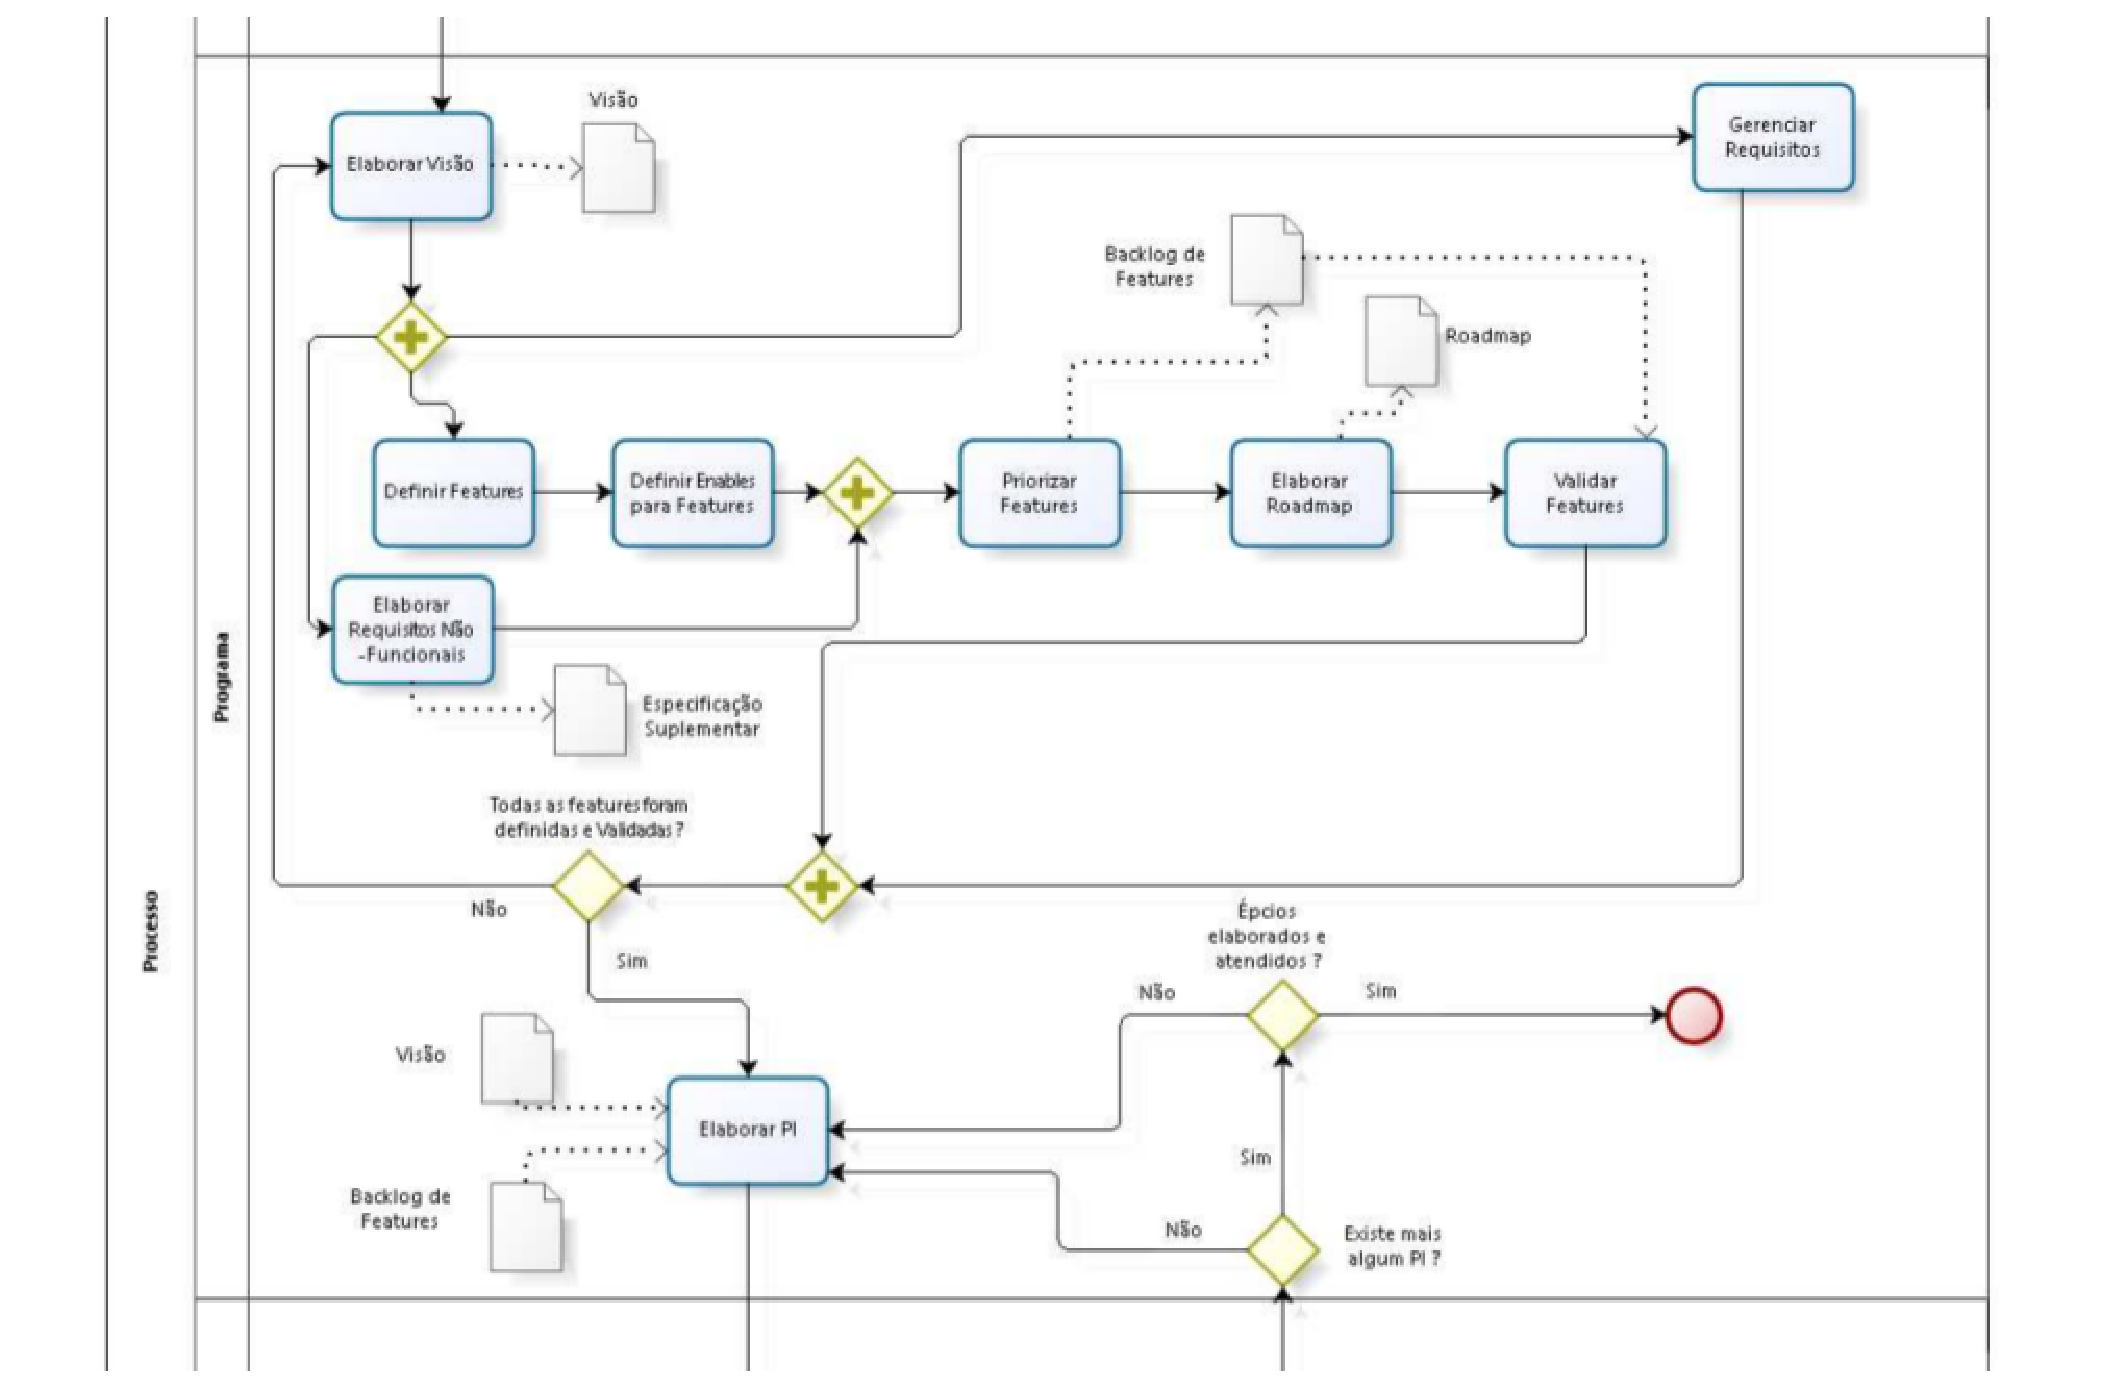
\includegraphics[keepaspectratio=true,scale=0.5]{figuras/nivelProgramaRequisitos.eps}
    \caption{Figura Nível de Programa}
\end{figure}

\subsection{Requisitos Não Funcionais}
Requisitos de Portabilidade: O sistema deverá ser executado em computadores ou celulares com suporte a navegadores. Os navegadores que irão suportar o site serão: Google Chrome, Internet Explorer, Mozilla Firefox e Safari.\\
\tab Requisitos de Implementação: O sistema deverá ser desenvolvido em Ruby com o Framework Rails.\\
\tab Requisitos de Eficiência: O sistema deve processar todas as requisitos no menor tempo possível.\\
\tab Requisitos de Confiabilidade: O sistema deve ficar 24 horas por dia durante toda semana disponível.\\

\subsection{Features Identificadas}
O Backlog de Features ficou composto pelas seguintes features:\\
1. Feature 1 (E1F1) – Sistema de Pedidos\\
\tab Descrição: O sistema de pedidos do sistema deve efetuar o pedido de forma totalmente autônoma, integrado com o banco de dados do sistema  e efetuar o pedido conforme o endereço passado pelo cliente com a forma de pagamento escolhida também por ele, tendo um feedback tanto para o cliente quanto para o administrador que recebe os pedidos.\\
\tab Obs: Os endereços de entrega podem ser:\\
\tab Residenciais - onde o cliente opta por receber os produtos em domicílio.\\
\tab Comerciais - onde o cliente que revende o produto deseja receber no próprio comércio.\\
\\
2. Feature 2 (E1F2) – Gestão de Usuários\\
\tab Descrição: Compradores são definidos segundo o tipo de pedidos que fazem:\\
\tab - Comprador Web: O usuário que faz pedidos pela plataforma web;\\
\tab - Comprador Direto: Aquele que compra diretamente com o Cliente;\\
\tab - Business to Business (BtoB): Empreendedores que compram grandes quantidades de produtos e os revende.\\
\\
3. Feature 3 (E1F3) – Gestão de Produtos\\
\tab Descrição: A Gestão de Produtos deve gerir os produtos envolvidos na Fabrica de Massas do Chef Nery, sendo integrado com o banco de dados do sistema. Além disso informar o valor de cada produto e gerar informações relevantes de acordo com o tempo acerca dos produtos.\\
\\
4. Feature 4 (E2F4) – Divulgar Canais de Comunicação\\
\tab Descrição: Disponibilizar informações do whatsapp e facebook da empresa a partir do site da empresa.\\

\subsection{Roadmap}
O Roadmap tem como objetivo apresentar um conjunto de releases planejadas com suas respectivas datas, features e priorizações baseadas no tempo. É elaborados para estabelecer uma estratégia de entrega para atingir metas e mostra como se dará a evolução do trabalho como um todo. O Roadmap também pode ser definido como uma série de releases planejadas em datas, em que cada uma possui uma lista de features priorizadas (LEFFINGWELL, 2011).\\
\tab No trabalho foi definido um conjunto de atividades relacionados a todo o processo assim como suas respectivas datas de entregas. A partir das prioridades definidas em conjunto com o cliente, as features foram dispostas como figura do Roadmap.\\
\begin{figure}[h]
    \centering
    \label{fig01}
        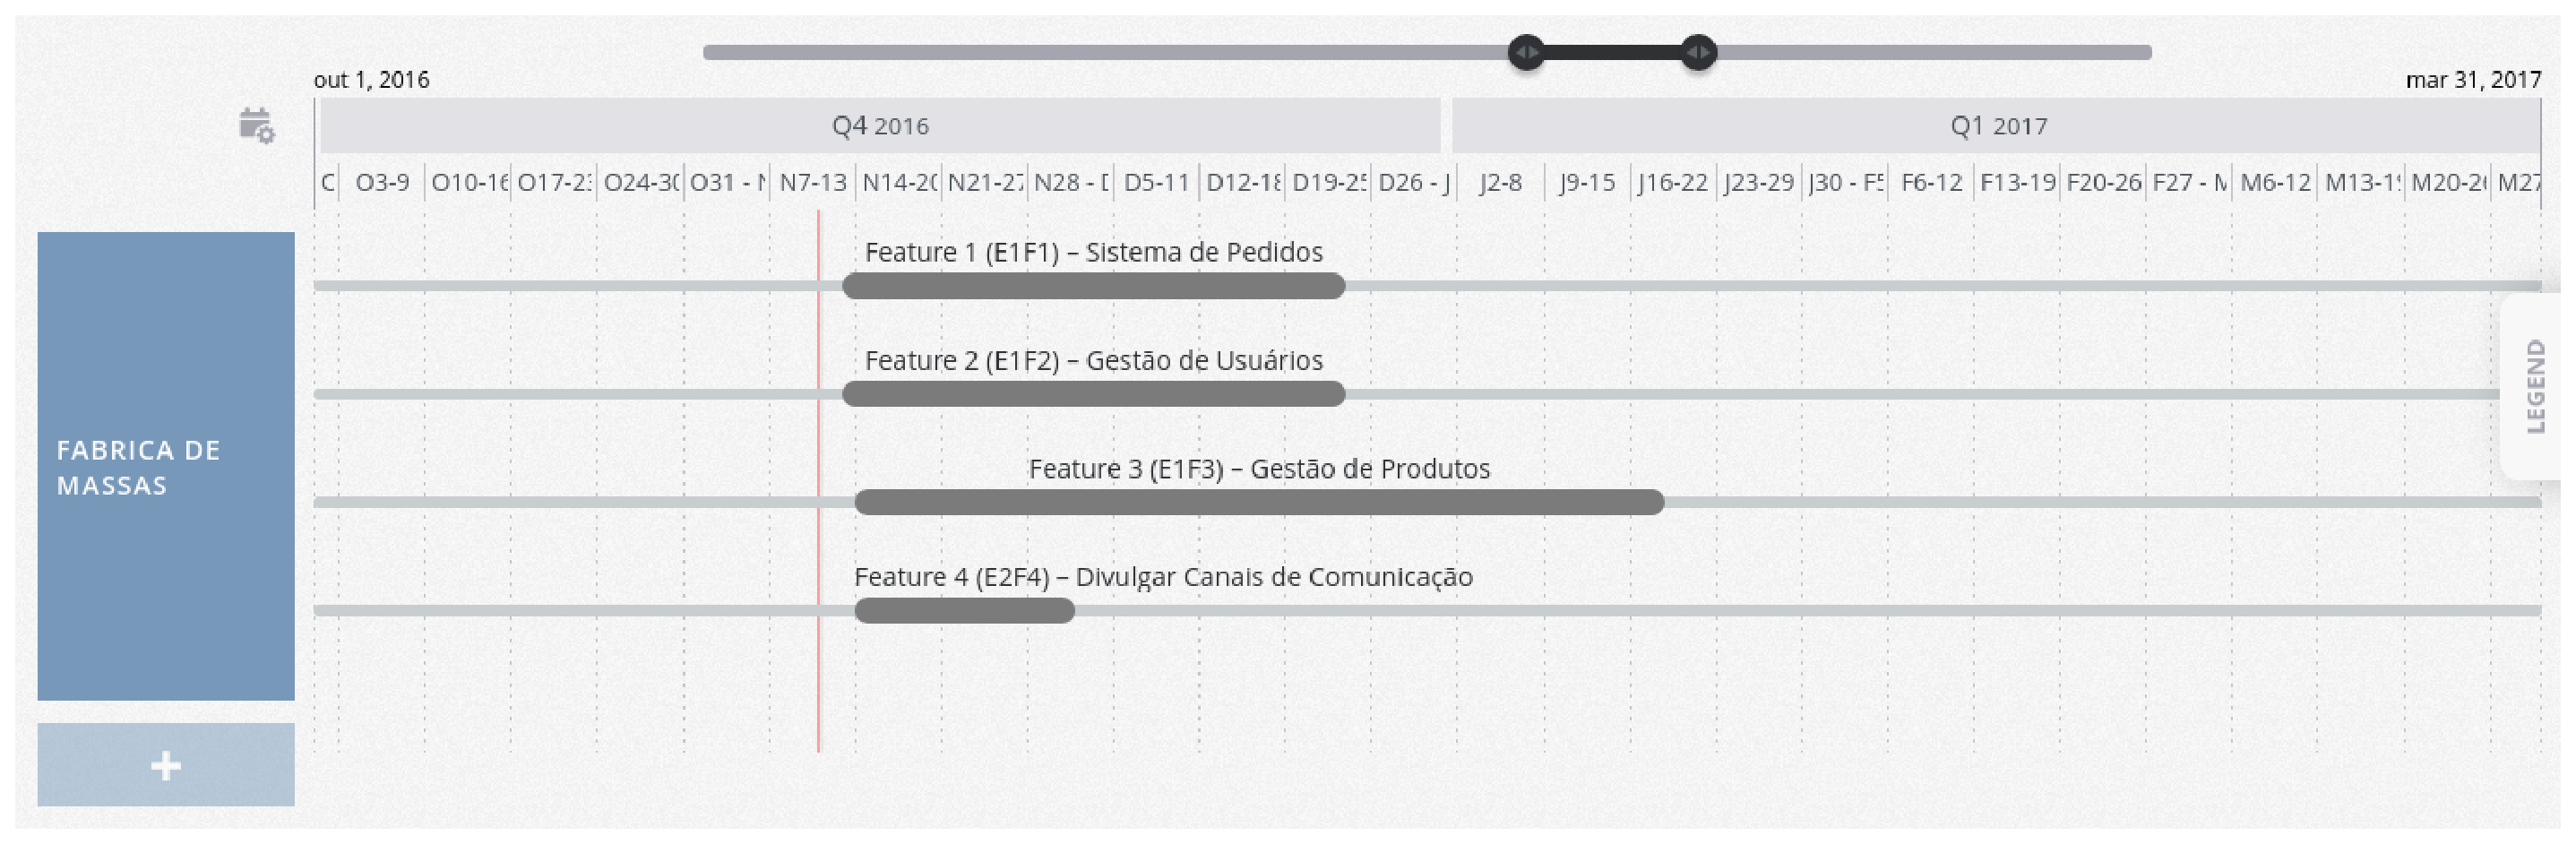
\includegraphics[keepaspectratio=true,scale=0.3]{figuras/roadmunk.eps}
    \caption{Figura RoadMap - Elaborado no Software Roadmunk}
\end{figure}
\\
\tab No Roadmap foram definidas 4 features a serem implementadas, elas serão elaboradas de acordo as com histórias de usuário que foram priorizadas, portanto, o desenvolvimento de cada Sprint se dará de acordo com o que agrega mais valor ao cliente, que são as seguintes características:\\
\tab - Divulgar Canais de Comunicação;\\
\tab - Cadastrar Produto (Divulgação do produto incluindo descrição);\\
\tab - Emitir Pedido mesmo que não seja utilizado sistemas de pagamento via internet.\\
\\
Essas características priorizadas serão definidas no tópico de Nível de Time em forma de Histórias de Usuário com mais clareza.\\

\section{Nível de Time}
Este nível se assemelha bastante ao SCRUM,  portanto existem algumas atividades, tais como: Sprint Planning, Sprint Review, Sprint Retrospective. Nesta etapa, as Features são fragmentadas em Histórias do Usuário. Esta etapa está relacionada com o desenvolvimento dos PI’s.\\
\tab As Atividades que constituem o Nível de Time são:\\

- Definir Histórias do Usuário;\\
\tab - Priorizar Histórias do Usuário;\\
\tab - Sprint Planning;\\
\tab - Implementar Código;\\
\tab - Sprint Review;\\
\tab - Sprint Retrospective;\\
\tab - Gerenciar Requisitos.\\

\begin{figure}[h]
    \centering
    \label{fig01}
        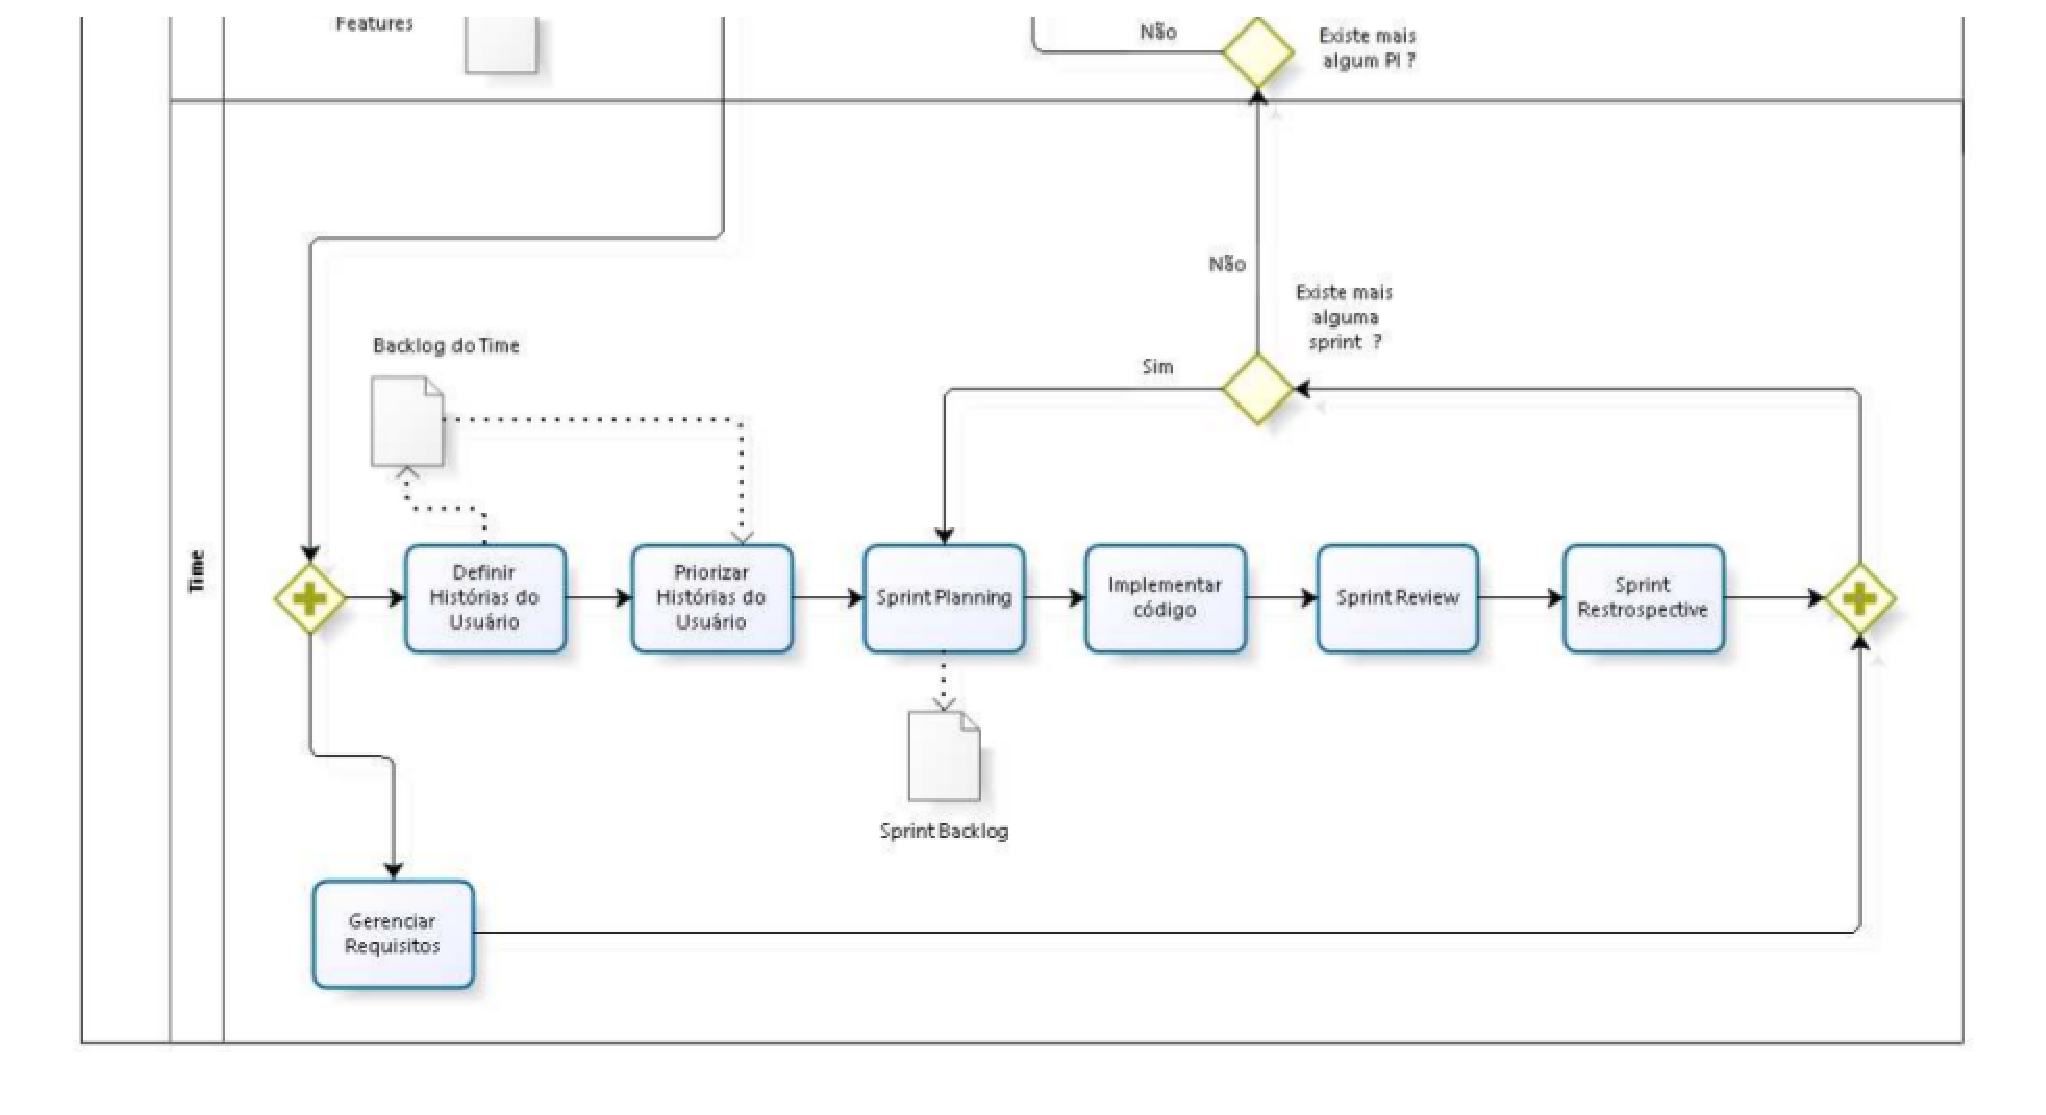
\includegraphics[keepaspectratio=true,scale=0.5]{figuras/nivelTimeRequisitos.eps}
    \caption{Figura Nível de Time}
\end{figure}

\subsection{Backlog do Time}
O Backlog de time contêm as Histórias de usuário que serão desenvolvidas nas Sprints. As Histórias de Usuário segue o seguinte modelo:\\
\\
\tab Como <Ator> desejo <Ação> para <Funcionalidade>\\
\\
\tab O Ator pode ser definido como proprietário, de uma forma mais simples: o usuário, o interessado na funcionalidade. Definir o ator de uma forma específica ajuda a identificar o contexto do uso do sistema.\\
\tab A Ação trata do que o Ator deseja fazer para atingir o seu objetivo dentro do software em questão.\\
\tab A Funcionalidade condiz com o resultado esperado pelo Ator ao realizar uma devida ação. É o resultado do que foi feito.\\
\tab Os Pontos das Histórias de Usuário serão definidas no decorrer do desenvolvimento. As histórias de Usuário são:\\
\\
F1H1 - Pagar no ato da entrega \\
\tab Eu como cliente desejo efetuar a compra, pegando somente na hora da entrega, a fim de pagar por dinheiro ou por cartão.\\
\tab Depende de: Efetuar Pedido Checando o Estoque, Cadastrar Usuário, Escolher Endereço de Entrega, Manter Produto, Calcular Valor do Produto.\\





\section{Gerência de Mudanças}
\section{Rastreabilidade}

A rastreabilidade dos requisitos está diretamente ligada para referenciar um grupo coletivo de requisitos baseada em seus relacionamentos (GENVIGIR, 2009), ela estabelece formas de analisar o quanto mudanças afetaram o sistema.
Os elementos para estabelecer os relacionamentos entre os artefatos de software e os requisitos são chamados de elos, estes são elementos que são necessários para estabelecer a Rastreabilidade (GENVIGIR, 2009) e a partir deles pode ser levada em consideração um aspecto fundamental para esse contexto: a habilidade de descrever a “vida” de um determinado requisito. \\
O conceito de Rastreabilidade também pode ser definido como a capacidade de descrever e seguir o ciclo de vida de um requisito em diferentes direções (GOTEL, 1997). Com isso os mais diversos requisitos e seus elos com determinados artefatos pode-se criar uma teia de relacionamentos em que a rastreabilidade tem como característica acompanhar justamente esses relacionamentos.\\
Para este projeto foi escolhida a técnica vertical em que tem como característica relacionar artefatos dependendo de modelos. Para isso a rastreabilidade vertical será feita para Temas de Investimento, Épicos e Features e Casos de Uso.\\



\section{Atributos dos Requisitos}
Os requisitos do projeto irão ter alguns atributos que irão auxiliar no acompanhamento e gestão dos mesmos. Os atributos serão:\\
\tab \textbf{Data de criação do requisito:} quando o requisito foi criado na ferramenta;\\
\tab \textbf{Início previsto:} previsão de quando o requisito será desenvolvido;\\
\tab \textbf{Término Previsto:} previsão de quando irá terminar o desenvolvimento do requisito;\\
\tab \textbf{Data de início efetivo:} data em que foi iniciado o desenvolvimento do requisito;\\
\tab \textbf{Data de conclusão do requisito:} quando o requisito terminou de ser desenvolvido;\\
\tab \textbf{Valor para o negócio:} será classificada a relevância para o projeto o requisito em Alta, Média e Baixa:\\
\tab - Prioridade Alta: É um requisito fundamental para a solução, o não atendimento desse requisito não atende a necessidade do cliente.\\
\tab - Prioridade Média: É um requisito importante, porém a nível de satisfação do cliente mas não algo que é indispensável para a solução.\\
\tab - Prioridade Baixa: É um requisito que seria bom ter, mas não agrega valor a solução e pode ter seu desenvolvimento adiado.\\
\tab \textbf{Status do Requisito:} verifica a condição atual do requisito:\\
\tab - Temas de Investimento e Épicos: podem estar nos estados Novo, Em Progresso e Feito.\\
\tab - Features e Casos de Uso: podem estar nos estados Aberto, Em Progresso, Em Teste e Feito.\\
\tab \textbf{Esforço:} Será uma característica que irá indicar o quanto um requisito toma de esforço para ser concluído. Para isso será utilizado o Planning Poker, em que os envolvidos devem pontuar o quanto toma de esforço um requisito até chegarem a um consenso.\\
